\chapter{模块介绍}
这一章节主要介绍软件的开发过程,将软件按照功能逐步地进行细致划分,从而完成软件的设计任务。
\section{软件框图}
如 \figurename{} \ref{fig:softarch} 为软件整体的关系图。
\begin{figure}[h]
	\centering
	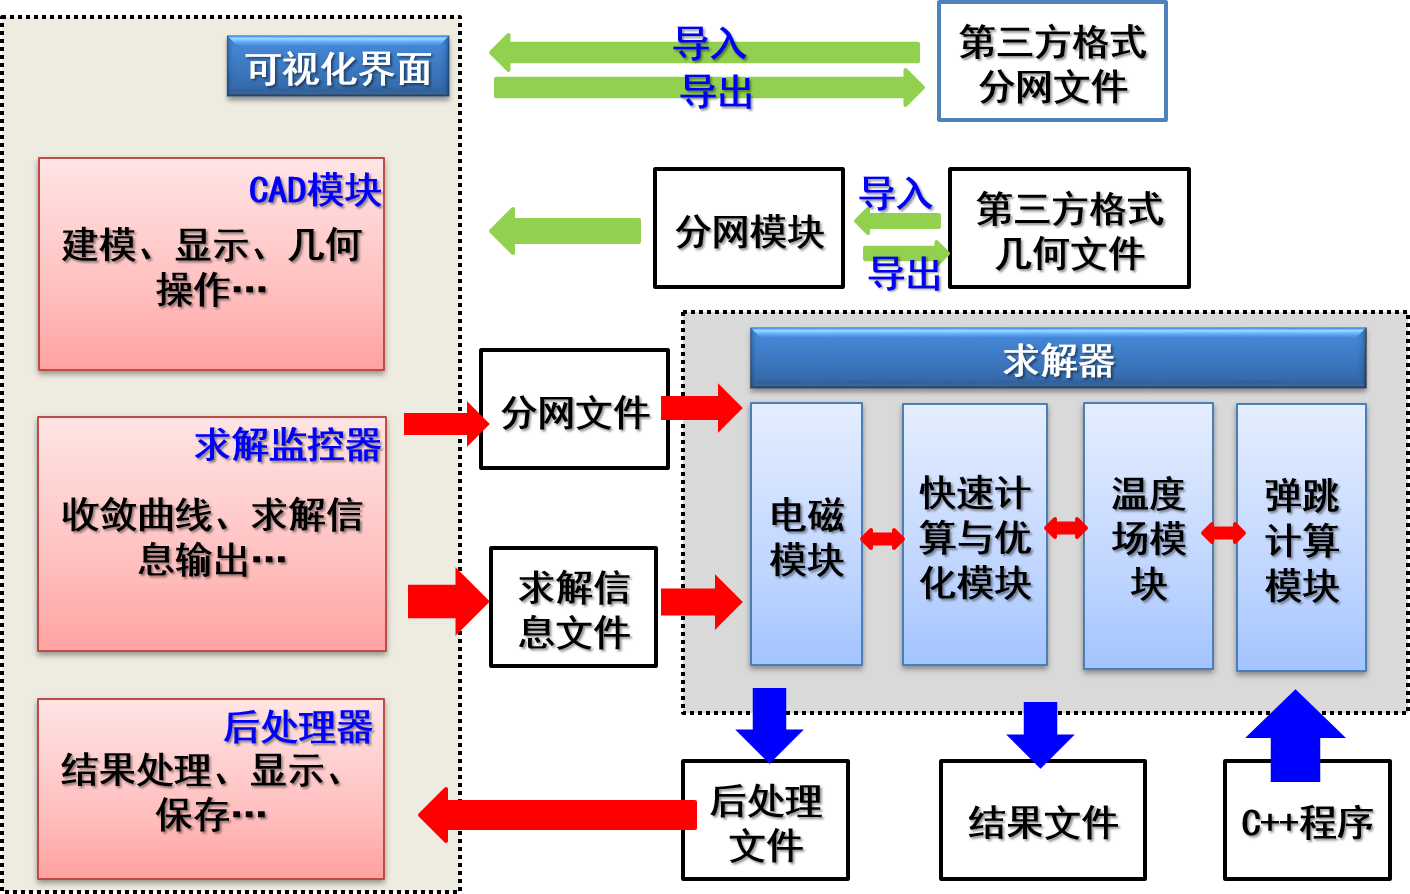
\includegraphics[width=0.7\linewidth]{figures/softarch}
	\caption{软件FEEM整体设计框架}
	\label{fig:softarch}
\end{figure}

\subsection{磁场问题的有限元求解}

\subsubsection{静磁场}

\subsubsection{瞬态磁场}
在电器当中的瞬态问题,主要还是考虑到可动部件的运动。

静态特性

在静态特性计算当中,可运动部件并没有真的在运动。只不过相对固定部分发生一定的位移之后,计算出电磁场的分布。求解的是一组静磁场问题。也没有考虑任何的动态方程,等同于针对位移的参数求解。

动态特性

实际的仿真过程需要考虑运动的耦合。电磁-运动的耦合是一种电磁问题和运动学问题的弱耦合。在每一个时间步的计算当中,先求解电磁场问题,然后再求解运动学问题,求解过程如下:

1.求解麦克斯韦方程组,计算发生一定位移后,施加在运动部件上的电磁力或电磁力矩;

2.求解运动部件的动态方程,计算出运动部件在时间步内的加速度值和速度,并且计算出下一时间步时运动部件新的位移位置;

3.将运动部件移动到新的位置,并且进行重分网操作;

4.返回步骤1。

\subsection{电磁力的计算}

Arkkio’s method


各种方法的优缺点对比

stress tensor方法的缺点

在数学上,这种方法是完全正确的,能够得到准确的力矩值,前提是B的计算值是准确的。然而,通常情况下不是这样的。需要注意的是,有限元求解是一种数值计算方法,因此,我们大多数情况下处理的都是近似值。特别地,我们实际求解得到的是磁势向量A,而磁感应强度B是通过计算A的旋度来得到的。这实际上是一个微分过程,如果我们对某些不准确的变量进行了微分操作,那么最后得到的计算结果必然也是有误差的。也就是说,我们计算得到的B的误差将会比A的误差更大。如果能够取消这个微分计算的过程,那么将有可能提高计算精度。
\subsection{优化问题}

\section{界面设计}

\subsection{Ribbon模块}
Ribbon模块是一个能够提供类似Office界面风格的组件。同时,COMSOL采用的也是类似界面。

1.如何自定义Ribbon的主题?
\subsection{QtFLEX模块}
该模块实现类似Visual studio当中的可停靠用户界面的组件。窗口内部的子部件可以根据用户随意的进行位置放置。可以设置自动隐藏停靠,可以与其他窗口进行分割,合并。
\begin{figure}
	\centering
	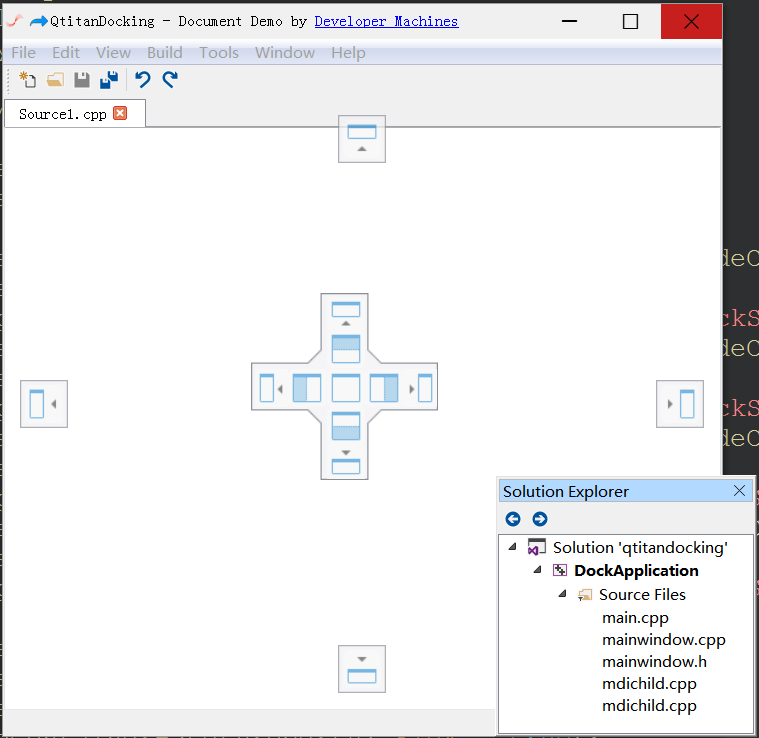
\includegraphics[width=0.7\linewidth]{figures/dock}
	\caption{Dock演示}
	\label{fig:dock}
\end{figure}

\subsection{界面布局}

\section{定义}
为了对数据进行存储,需要定义合理的格式和存储方式。
\subsection{工程文件格式及存储}
工程文件,即是软件会打开的文件,通过读取这个文件,软件可以获得该项目当中的几何模型、物理设置参数、分网信息、求解信息等。目前,最普遍的方式就是采用标记式语言进行存储,首选XML语言。
\subsection{几何文件格式及存储}
几何图形是用户在操作软件过程当中一直会使用到的东西,所以这部分数据肯定是常驻内存。在软件的核心,需要定义几何存储的格式来代表各种图形,这些图形可以是用户自己创建的,也可以是不同格式的几何文件转换过来的。
\subsection{分网文件格式及存储}
跟几何文件类似,也需要在工程内部自定义分网数据格式,来保存从各种格式的分网文件读取并转换而来的数据。
\subsection{结果数据文件及存储}
在求解结束后,需要一个数据结构来存储计算得到的各种数据结果。
\subsection{编程代码规范}
为了使软件开发尽量的规范,开发小组成员应当遵守以下操作:
\section{CAD绘图}
几何绘图是软件可视化最重要的一个部分。
\subsection{绘图原理}
在显示屏上你所看到的有趣的东西,都是程序员尽力地让一切看起来都跟真的似的,实际上,它依旧还是冷冰冰的机器,只是用的时间长了可能会发热而已。
\subsection{基本几何形状}
需要实现的基本几何形状有:点、线、圆弧、长方形等。
\subsection{形状操作}
所谓的用户能够对显示的几何形状进行控制,实际上是程序针对用户的鼠标操作与实际几何形状的位置进行了比较计算之后,进行了一些算法。每一次改变都会导致显示内容的刷新,只不过肉眼无法辨别出来。
\subsubsection{形状选中、调整大小、删除、隐藏显示}

\subsubsection{自动吸附}

\subsubsection{布尔操作}

\subsubsection{缩放、变形}

\subsection{与分网显示、后处理的接口}

\subsection{参数绘图}

\section{材料库}
为了对模型当中的结构添加相应的材料属性,需要提供一个材料管理器的功能,能够存储一些常见的材料,并且能够实现新建、修改、删除等操作。
\subsection{已有材料库}

\subsection{新建、删除材料}

\subsection{导入、导出材料}

\section{分网生成}
分网无疑是有限元器求解最为关键的步骤之一。
\subsection{分网读取、导出}

\subsection{有限元分网形状}

\subsection{读取几何模型并分网}

\subsection{分网控制}

\subsection{删除分网}

\subsection{分网可视化}

\section{求解器}

\subsection{求解器设置}

\subsection{优化模块}
当所有的求解信息都设置好后,不仅可以实现磁场的求解,还能够实现对某些参数的优化设计。

\subsection{收敛曲线显示}

\section{后处理}
求解器计算得到的结果无疑要使用最好的方式展现给用户。
\subsection{结果曲线}

\subsection{结果云图}

\subsection{结果矢量图}

\subsection{数据导出}